\documentclass{article}

% NeurIPS 2026 style file: obtain neurips_2026.sty from the official Overleaf template
% ("Formatting Instructions For NeurIPS 2026", Open as Template) and place it beside this file.
% The style file is not modified or redistributed here.
% "preprint" prints the author name (default option anonymises and adds line numbers) and adds the
% footer "Preprint. Work in progress." TODO(OWNER): confirm this option is acceptable to the instructor.
\usepackage[preprint]{neurips_2026}

\usepackage[utf8]{inputenc}
\usepackage[T1]{fontenc}
\usepackage{hyperref}
\usepackage{url}
\usepackage{booktabs}
\usepackage{tabularx}
\usepackage{amsfonts}
\usepackage{amsmath}
\usepackage{nicefrac}
\usepackage{microtype}
\usepackage{xcolor}
\usepackage{graphicx}

\newcolumntype{Y}{>{\raggedright\arraybackslash}X}
\newcommand{\owner}[1]{\textcolor{red}{\textbf{[OWNER: #1]}}}

\title{Flat, Tiered or Graph? How the Structure of a Specification
Changes the Code Written by AI}

\author{%
  Victor Truong \\
  Student number 300264088 \\
  MIA 5150, University of Ottawa \\
  ntruo093@uottawa.ca \\
}

\begin{document}

\maketitle

% ------------------------------------------------------------------ 1
\section{Project Category}

Its category is \emph{benchmark and empirical study}: a controlled comparison of three ways of
presenting the same specification to the same coding agent.

% ------------------------------------------------------------------ 2
\section{Testable Claim}

We claim that \textbf{an AI coding agent produces code of higher quality from a structured, graph-based
specification than from the same specification given as a single long flat prompt or as tiered
spec-driven-development (SDD) files}, and we will show it by measuring \textbf{code quality, hallucination
and specification omission}, on \textbf{our own feature-implementation tasks and an AI-coding benchmark}.

% ------------------------------------------------------------------ 3
\section{Problem and Motivation}

Coding agents are increasingly asked to build software from written specifications. The specification
is usually supplied either as one long prompt (vibe coding) or as a folder of tiered Markdown files,
the layout of the spec-driven-development (SDD) method. Long inputs are not used evenly: models use
information at the beginning and end of a long context better than information in the middle \citep{liu2024lost},
so a requirement buried in a long specification may be dropped or replaced by what the model finds typical.
Tiering the files helps but does not remove the difficulty, because contradictions and duplication across files remain.
A further step is to compile the specifications into a \emph{graph} of small requirement nodes with terms and links, so that the
agent receives a checklist, a vocabulary and the relations between requirements.

Whether this additional structure improves the generated code, or merely adds cost, has not been tested.
We compare the three representations while holding everything else fixed. A null result would still be a
finding, and the agent's own list of what it had to invent would show what a specification graph must carry.

% ------------------------------------------------------------------ 4
\section{Related Work}\label{sec:related}
The related literature (scoring of generated code, hallucination in generated code, long-context effects, prompt-format effects, and evaluation statistics) is reviewed in Appendix~\ref{app:related}.

% ------------------------------------------------------------------ 5
\section{Proposed Approach}

\subsection{Models}
Claude Haiku, Claude Sonnet and Claude Opus are used through Claude Code.
No local or open-weights model is used, so no GPU is required.

\subsection{Data and Tasks}

\textbf{Main study: our own tasks.} A small set of feature-implementation tasks written by us. Each has a specification,
a hidden test suite and a numbered requirement list, and is packaged as one task per directory so that any candidate
evaluation platform can run it. The same content is rendered in three specification formats.

\textbf{External validity: one public benchmark.} One public benchmark whose task text is a specification, re-rendered in the
same three formats. The candidates are ProjectEval \citep{liu2025projecteval} (input levels: prompt, checklist and code skeleton),
RealBench \citep{li2026realbench} (text requirements plus UML) and Doc2Feat-Bench \citep{jiang2025doc2feat}; the choice depends on
licence, size and whether task inputs can be replaced.

\textbf{Evaluation platform (undecided).} ProjectEval, RealBench or Harbor \citep{harbor_docs}; one will be selected in week~5.
Harbor packages custom tasks and records per-trial time, cost, tokens and retries, whereas ProjectEval and RealBench are correctness
benchmarks. Efficiency metrics are taken from Claude Code's own logs whichever platform scores correctness.

\textbf{Study artifact.} For each task the same specification content is supplied in three formats.
\emph{Flat}: one long Markdown file in a fixed order.
\emph{Tiered}: the SDD layout, with a short vision and rules file and one file per feature.
\emph{Graph}: the same content compiled by the SDD Compiler into a graph of requirement nodes, terms and links, read by the agent as files.

\subsection{Experimental Variables}
\begin{itemize}
  \item \textbf{Varied, specification format:} flat, tiered, graph.
  \item \textbf{Varied, agent:} Haiku, Sonnet, Opus.
  \item \textbf{Hypotheses:} the graph ties with flat and tiered on clean, single-file specifications and helps on messy,
        multi-file specifications (duplicates, scattered refinements, contradictions); these are design judgements, not results. The smaller model gains more
        than the larger one (ClassEval). Our own tasks include both clean and messy specifications.
  \item \textbf{Fixed:} the task text, the tool list and permission mode, an empty output
        directory, the model identifier and effort, and the turn cap.
  \item \textbf{Repetitions:} two per (task, specification format, agent) as a design value.

\end{itemize}

% ------------------------------------------------------------------ 6
\section{Baseline and Trial-Run Result}

\textbf{Trial run: the real graph of our own software.} We compiled this project's specification set with the SDD Compiler. The input is nine Markdown files: a vision, a constitution, a README and six feature specifications, one folder per feature.
The compilation turned 845 text blocks into \textbf{933 requirement nodes in 374 families},
using 3\,507 model calls (2\,673 plus 834 for later fixes), and 9.05~h for the first compilation.
This graph is shown in Appendix~\ref{app:graph}.

% ------------------------------------------------------------------ 7
\section{Evaluation Plan and Metrics}\label{sec:eval}

Four groups of measures will be examined.
\begin{enumerate}
  \item \textbf{Code quality:} hidden tests passed, together with the measures in Table~\ref{tab:quality}.
  \item \textbf{Hallucination:} invented requirements and invented libraries or interfaces, using the measures in Table~\ref{tab:halluc}.
  \item \textbf{Specification omission:} the share of numbered requirements that the code does not implement, using the measures in Table~\ref{tab:omission}.
  \item \textbf{Efficiency:} completion time, estimated API-equivalent cost, input and output tokens, files read and edited, failed commands and number of tries,
        taken from Claude Code's own logs, to show whether the graph helps or slows the agent.
\end{enumerate}
The candidate measures found in the literature are listed in Tables~\ref{tab:quality}--\ref{tab:omission} in Appendix~\ref{app:measures}.

% ------------------------------------------------------------------ 8
\section{Compute Budget}

No GPU is required: all models are hosted, so the course limits of about 15\,GB per job and 20 GPU-hours do not apply.

% ------------------------------------------------------------------ 9
\section{Week-by-Week Plan}

\begin{table}[h]
  \caption{Plan by week.}\label{tab:plan}
  \centering\small
  \begin{tabularx}{\linewidth}{@{}p{0.07\linewidth}p{0.14\linewidth}Y p{0.09\linewidth}@{}}
    \toprule
    Week & Dates & Task & Who \\
    \midrule
    4 & to 2 Oct & Proposal; compile the real graph (done); shortlist public benchmarks & Victor \\
    5 & 5--9 Oct & Select the evaluation platform among ProjectEval, RealBench and Harbor (can it score a Claude Code project? which per-trial fields?); choose tasks; write the requirement lists; build the three renderings and the parity check & Victor \\
    5 & 5--9 Oct & Run harness (headless runs, test runner, logs) & Victor \\
    6 & 12--16 Oct & Pilot: one run per specification format per model; measure calls and dollars per run; fix the number of repetitions & Victor \\
    7--8 & 19--30 Oct & Main runs, interleaved across days; run the scoring scripts after each & Victor \\
    7--8 & 19--30 Oct & Blind omission audits; re-label a sample to measure agreement & Victor \\
    9 & 2--6 Nov & Analysis; \textbf{progress check-in, 6 Nov} & Victor \\
    10 & 9--13 Nov & Hallucination counts; list of what the agents invented & Victor \\
    11 & 16--20 Nov & Draft report; slides & Victor \\
    12 & 23--27 Nov & Rehearsal; \textbf{presentation, 27 Nov} (or 4 Dec) & Victor \\
    13 & 30 Nov--4 Dec & Final report (six pages), README with seeds and reproduction steps & Victor \\
    \bottomrule
  \end{tabularx}
\end{table}

% ------------------------------------------------------------------ 10
\section{Risks and Smaller Backup Project}\label{sec:risks}

\begin{itemize}
  \item \textbf{Platform undecided.} ProjectEval and RealBench may not accept projects produced outside their own pipeline (unconfirmed); Harbor's Claude Code agent must work with the subscription login.
  \item \textbf{Benchmarks may not fit.} Popular coding benchmarks (HumanEval, SWE-bench) do not ship specifications that can be rendered in three formats; Doc2Feat-Bench is the
        candidate found so far, and its licence, size and ease of execution are not yet checked. If none fits, the plan falls back to the backup below.
  \item \textbf{Compilation cost of the graph format.} Every task's specification must be compiled; the measured cost of one full compilation (Section~6) is large, and small tasks may cost far less. To be measured.
  \item \textbf{Compiler gaps.} The graph may lose content; this is scored as omission of the graph format and reported.
  \item \textbf{Variance.} Runs are stochastic and two repetitions may be too few; results are reported as intervals, and a null result is valid.
  \item \textbf{Audit load.} The audit sample may be reduced to 10 per run.
\end{itemize}

\textbf{Smaller backup project.} Two specification formats (tiered versus graph), Haiku and Sonnet only, 3 tasks and 3 repetitions on a small hand-picked specification set, with omission rate as the primary metric:
$3 \times 2 \times 2 \times 3 = 36$ runs (design value), without Opus and without the flat format.

% ------------------------------------------------------------------ references
{\small
\bibliographystyle{plainnat}
\bibliography{references}
}

% ------------------------------------------------------------------ appendix
\appendix
\section{Snapshot of the Compiled Graph}\label{app:graph}

Figure~\ref{fig:graph} is a screenshot of the HTML viewer written by the compiler for the 933-node graph of Section~6.

\begin{figure}[h]
  \centering
  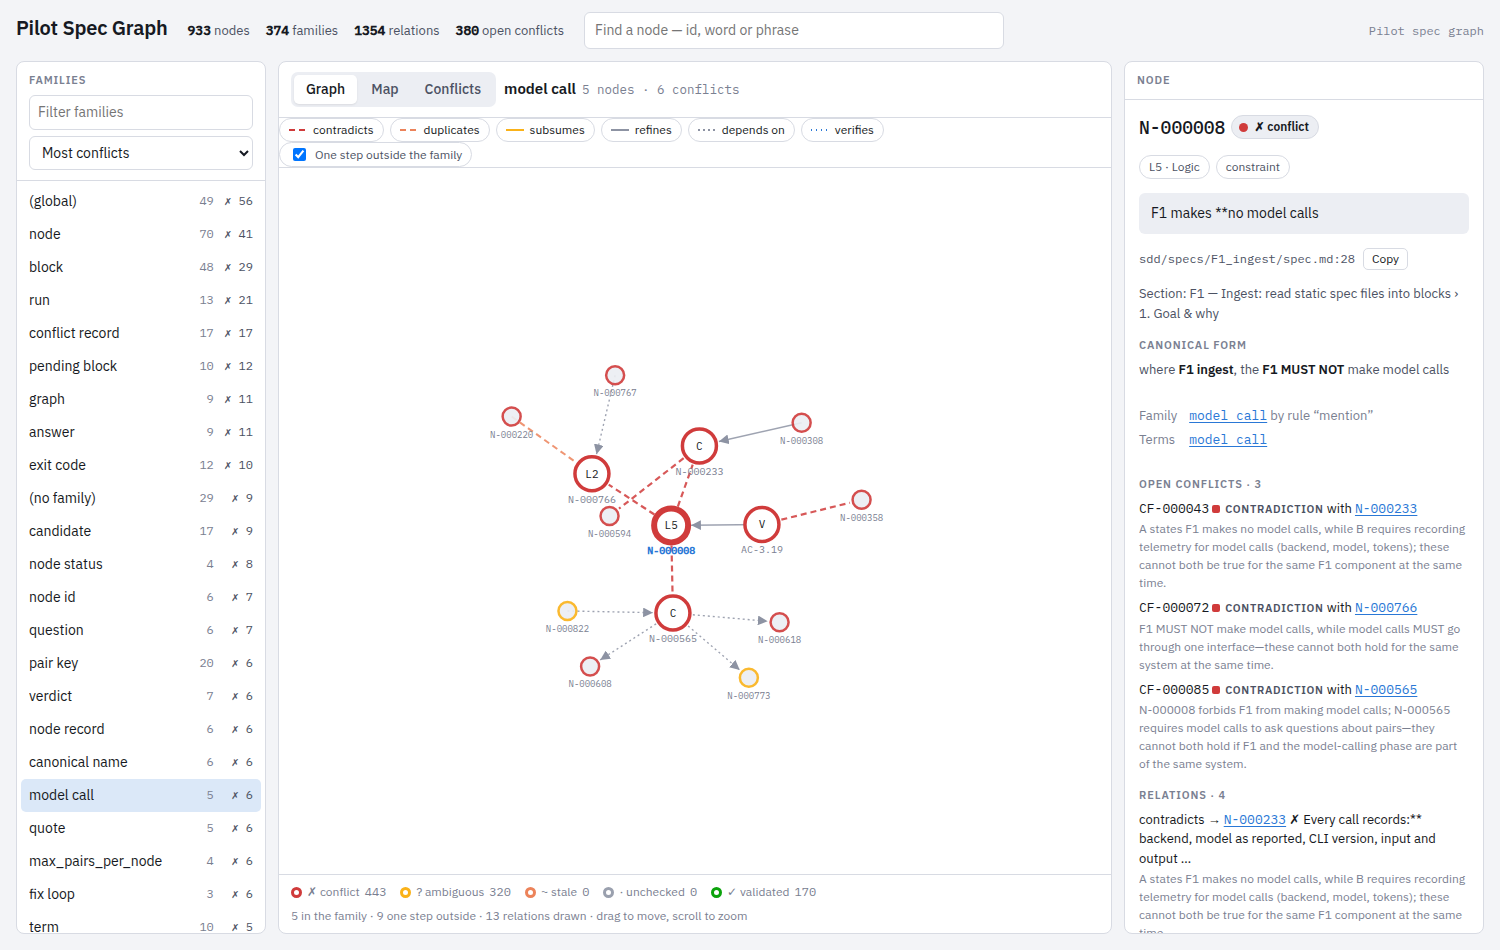
\includegraphics[width=\linewidth]{graph-snapshot.png}
  \caption{Snapshot of the compiled specification graph (frozen pilot graph).}\label{fig:graph}
\end{figure}

\section{Candidate Measures from the Literature}\label{app:measures}

Tables~\ref{tab:quality}--\ref{tab:omission} list the candidate measures for code quality, hallucination and specification omission (Section~\ref{sec:eval}).

\begin{table}[h]
  \caption{Candidate measures of code quality.}\label{tab:quality}
  \centering\small
  \begin{tabularx}{\linewidth}{@{}p{0.22\linewidth}Y p{0.2\linewidth}@{}}
    \toprule
    Metric & What it measures & Source \\
    \midrule
    pass@$k$ & Share of tasks with at least one of $k$ samples passing all tests & \citet{chen2021codex} \\
    Resolved rate & Share of tasks whose patch makes the designated failing tests pass without breaking others & \citet{jimenez2024swebench} \\
    Test-suite strength & Stronger tests lower measured pass rates: HumanEval+ has about $80\times$ more tests and pass@$k$ falls by 19.3--28.9\,\% & \citet{liu2023evalplus} \\
    Efficiency of generated code & Speed of generated code (EvalPerf) & \citet{evalplus_repo} \\
    Non-functional quality (security, maintainability, performance efficiency; ISO/IEC 25010) & A gap between what research measures and what practitioners value (maintainability, readability); prompting alone did not reliably improve these & \citet{sun2025quality} \\
    Similarity to a reference (BLEU-like, AST similarity, Token F1) & Used beside execution in ProjectEval; Token F1, AST similarity and syntax validity in the portability study & \citet{liu2025projecteval,grynets2026portability} \\
    LLM-as-judge quality & An LLM scores correctness or usefulness & \citet{zheng2023judge,crupi2025judge,kumarappan2026devbench} \\
    \bottomrule
  \end{tabularx}
\end{table}

\begin{table}[h]
  \caption{Candidate measures of hallucination.}\label{tab:halluc}
  \centering\small
  \begin{tabularx}{\linewidth}{@{}p{0.22\linewidth}Y p{0.2\linewidth}@{}}
    \toprule
    Metric or taxonomy & What it counts & Source \\
    \midrule
    HalluCode taxonomy & 3 primary and 12 specific hallucination categories in generated code, plus a benchmark & \citet{liu2024halucode} \\
    Practical-generation taxonomy & Taxonomy from six LLMs, with repository-level dependency context; retrieval-based mitigation & \citet{zhang2025hallucination} \\
    CodeHalu & Four types (mapping, naming, resource, logic), detected by execution-based verification; 8\,883 samples from 699 tasks & \citet{tian2025codehalu} \\
    Package hallucination rate & Share of suggested packages absent from the official registry; 576\,000 samples, 16 LLMs; about 5.2\,\% (commercial) and 21.7\,\% (open-source) as reported & \citet{spracklen2025package} \\
    Groundedness under unsatisfiable prompts & Whether the model fabricates or refuses when the task cannot be done; 270 prompts in six languages; Cohen's $\kappa$ 0.73 against human judgement & \citet{dasu2026refusing} \\
    Survey of taxonomies, benchmarks and metrics & Reviews taxonomies, benchmarks and mitigation & \citet{lee2025hallucination} \\
    SBC score & Reconstructs system requirements from generated code and compares them with the original specification; combines semantic similarity, BLEU and a completeness check; flags missing features and hallucinations & \citet{ponnusamy2025sbc} \\
    \bottomrule
  \end{tabularx}
\end{table}

\begin{table}[h]
  \caption{Candidate measures of specification omission (requirement coverage).}\label{tab:omission}
  \centering\small
  \begin{tabularx}{\linewidth}{@{}p{0.22\linewidth}Y p{0.2\linewidth}@{}}
    \toprule
    Metric & What it measures & Source \\
    \midrule
    SBC completeness & Missing features found by reverse-generating requirements from code and comparing them with the specification & \citet{ponnusamy2025sbc} \\
    Prompt Coverage Adequacy & How well a \emph{test suite} satisfies the requirements in a prompt, via LLM attention; reported to find over 30\,\% more faults than code coverage when guiding test generation & \citet{tambon2026prompt} \\
    API coverage & Share of specified endpoints implemented by the generated repository (up to 73.91\,\% reported) & \citet{peng2026repogenesis} \\
    Functionality coverage & Share of required functionality covered, reported beside pass rate & \citet{chen2026repo0} \\
    Requirement success with a traceability graph & Success rate on 125 use cases; a validator agent builds a graph linking requirements, design and code & \citet{chen2026tracedev} \\
    Omission as a specification defect & Conflict, omission and ambiguity as \emph{requirement} deficiencies, not code omissions & \citet{tian2026wisespec} \\
    \bottomrule
  \end{tabularx}
\end{table}

\clearpage % flush the three tables of Appendix B before Appendix C
\section{Related Work}\label{app:related}
% All papers were opened at their arXiv abstract page on 2026-09-29; full text was not read (see references.bib).

\textbf{Hallucination in generated code.} \citet{zhang2025hallucination} derive a hallucination taxonomy from six
LLMs and propose a retrieval-based mitigation. \citet{liu2024halucode} label 3\,120 code samples from four LLMs
on HumanEval and CoderEval (Cohen's $\kappa$ 0.76--0.96) and find that \emph{requirement conflicting} code, which does something
other than what was asked, is the largest class (39.60\,\%): the class a specification is meant to prevent.
\citet{spracklen2025package} report non-existent packages in about 5.2\,\% of samples for commercial models and 21.7\,\%
for open-source models, over 576\,000 samples, which provides an inexpensive automatic count of invented libraries.
We do not derive a new taxonomy; we count two narrow kinds, invented requirements and invented libraries or interfaces.

\textbf{Context position, length and distraction.} \citet{liu2024lost} show that models use information at the
start and end of a long input better than in the middle. This is the mechanism we expect to affect the flat
specification format, so the file order of that format is fixed and the position of each requirement is recorded.
Length alone also degrades performance: \citet{levy2024moretokens} report reasoning degrading at input lengths well
below the maximum; \citet{hsieh2024ruler} report that only half of 17 long-context models keep satisfactory performance
at 32K tokens; and \citet{shi2023distracted} show that irrelevant text in the prompt lowers accuracy.

\textbf{Unit size and how the agent reads.} ClassEval \citep{du2023classeval} finds every model much worse on whole
classes than on single functions, and that generating a whole class at once suits only the strongest models while
weaker models do better method by method. We adopt this as a hypothesis: the smaller Haiku model may gain more from a
graph that supplies one unit at a time than Opus does. SWE-agent \citep{yang2024sweagent} shows that a purpose-built
agent--computer interface changes the performance of the same model, so the layout of the files an agent reads is itself
a variable. Aider's repository map \citep{aider_repomap} gives the model a compact ranked overview so that it can
``figure out which files it needs to look at'', and GraphRAG \citep{edge2024graphrag} pre-computes summaries of clusters
in a graph to answer questions about a whole corpus; both are precedents for placing a map or graph between an agent and
a large body of text. Anthropic's guidance on context engineering \citep{anthropic2025context} likewise recommends keeping
light identifiers in context and loading detail just in time.

\textbf{Format as a confound.} \citet{he2024format} report up to 40\,\% variation for GPT-3.5-turbo on a code-translation
task across plain-text, Markdown, JSON and YAML templates, with larger models more robust; \citet{sclar2024format} report
differences of up to 76 accuracy points on LLaMA-2-13B from formatting changes alone. All three specification formats
therefore carry the same requirement text; only structure and layout change.

\textbf{Scoring of generated code.} \citet{chen2021codex} introduced HumanEval and the pass@$k$ metric for
functional correctness on short function-writing tasks. \citet{jimenez2024swebench} score whole-repository
edits by hidden tests on 2\,294 real GitHub issues (SWE-bench). Both measure whether the code passes tests
for one fixed task text. We keep tests but vary how the same requirements are represented, and we add counts
of omissions and hallucinations. \citet{liu2023evalplus} add about $80\times$ more tests to HumanEval and report
that pass@$k$ falls by 19.3--28.9\,\%, so a passing test suite alone is not accepted as a measure of quality;
we add an independent audit of omissions.

\textbf{Closest setting.} Doc2Feat-Bench \citep{jiang2025doc2feat} pairs a documentation change with the
corresponding implementation and developer tests, and reports that agents struggle with cross-file edits and
with interpreting documentation semantics. It fixes the documentation format and varies the agent; we fix the
agent and vary the representation of the specification.

\textbf{Judging and statistics.} \citet{zheng2023judge} document position, verbosity and self-preference biases of LLM
judges, with over 80\,\% agreement with human preferences for strong judges; LLM judging is therefore used only for triage and
is calibrated against human labels. \citet{miller2024errorbars} argues that evaluations should report error bars, paired
comparisons and planned power; we compare specification formats on the same tasks.

\end{document}
